\title{A Very Simple \LaTeXe{} Template}
\author{
        Vitaly Surazhsky \\
                Department of Computer Science\\
        Technion---Israel Institute of Technology\\
        Technion City, Haifa 32000, \underline{Israel}
            \and
        Yossi Gil\\
        Department of Computer Science\\
        Technion---Israel Institute of Technology\\
        Technion City, Haifa 32000, \underline{Israel}
}
\date{\today}

\documentclass[12pt, titlepage]{article}
\usepackage[utf8]{inputenc}
\usepackage[T1]{fontenc}
\usepackage{lmodern} % load a font with all the characters
\usepackage{graphicx} % includegraphics command is implemented here
\usepackage{float}
\usepackage{titlesec}
\newcommand{\sectionbreak}{\clearpage}

\begin{document}
\maketitle
\newpage
\begin{abstract}
Cafés are the home to many interesting ideas, it also a place where people go to meet new interesting people. In this report we discuss how a café environment can be realized online. The problem faced during the project includes overseeing, how one can look around and see other groups of people talking to each other. Overhearing, how one can listen to and find inspiration from other conversations going on in the café. Mingle, how one can move between these conversations in a subtle way.

A prototype was built using WebRTC, HTML5 and Javascript in order to solve these problems. Multiple solutions for each problem, together with a 2- and 3-dimensional views are being presented. The prototype consists of a video chat with multiple extra features for collaboration, like shared napkin to paint on and  synchronized YouTube watching, implemented to enhance the feeling of sitting at the same table. 
\end{abstract}
\tableofcontents
\clearpage
\section{Introduction}
A café is a very stimulating environment to many people. It’s a place where you can easily meet other interesting people. A place where you can walk by a table, overhear a conversation and oversee the whole café. We have all seen the group of girls sitting at a table drinking coffee and having conversations about anything, or the writer who finds inspiration for his next book from the environment and people around himself. Another scenario is all the people travelling to conferences each year. Businesses could save a lot of money if there existed a stimulating environment where one can meet people, collaborate in groups and mingle just like in the real world.

We want to transfer this feeling of being in a real café online. With the ability of seeing each other through video conference, collaborate together on a drawing, watch YouTube videos, reading pdfs together and of course being able to communicate through a text chat with all the participants sitting down at a table. Three other important aspects of transferring this feeling is overseeing, overhearing and mingling. These parts will be investigated and tested with a prototype.

When you are walking by a table in a real café you will hear what their conversation is about and also see all the participants, this is what we call overhearing and overseeing. Before you can sit down at a table and join a conversation you will gently ask if it is okay without trying to disturb their conversation too much.

The prototype contains a 2D- and 3D-view where overseeing, overhearing and mingling is realized.

\subsection{Problem description}
The problem we set out to solve was how to create a web based environment for sharing the feeling of being in a Paris Café including how to convey a feeling of overseeing, overhearing and mingling. Unlike traditional video chats where there is only one group of people participating, we want to create a video chat service with multiple rooms and multiple groups in each room. Where users can see the other groups and overhear conversations and move between the tables in an easy way.

Also how we can realize this feeling in a 2 and 3 dimensional view and still keep the café feeling, low latency so it feels like a real life meeting and present it all in a nice way in both views.
\subsection{Project goals}
The goal of the project is to:
\begin{itemize}
  \item Create a working prototype
  \item Implement some kind of overhearing
  \item Implement some kind of overseeing
  \item Implement some kind of mingle
  \item 2D and 3D view
  \item Evaluate the system with a user test
\end{itemize}
Implementing some kind of overhearing, overseeing and mingle is vague but here are some ideas for how it can be done.
\subsubsection{Overseeing}
How can one see the other participants at the same table while at the same time also see other groups of visitors in the same café. This could be realized with a 3D-environment with videos organized around different tables.
\subsubsection{Overhearing}
How can one hear the conversations from the other groups sitting at another table or just walking by that table. This could be realized with spatial sound in a 3D environment or by hover the mouse over a table in a 2D view.
\subsubsection{Mingle}
How can participants easily move between different conversations? I.e. if I oversee and overhear another interesting conversation, how can I gently move into that without too much interruption? This can be done by, for example, knocking, avatar gestures in a 3D world or writing a message to the group.

\subsection{Project requirements}
The project had a few restrictions of what technologies to use, WebRTC for media and data communication between clients, javascript and HTML5 for frontend. At the moment WebRTC is still under development. These technologies are used to promote using native browsers without any plugins.
\subsection{Project delimitations}
This is a big project and it need some limitations, it is our imagination and time that decides. We decided to limit us to have six cafés, six tables in each café and six persons at each table maximum. The server we are using have limitations and therefore the amount of people at each table is limited.
\subsection{Research questions}
The questions we want to answer is:
\begin{itemize}
	\item Does the ability to oversee other groups of people in the same virtual room affect the experience of online video chat?
		\begin{itemize}
			\item What is the effect?
		\end{itemize}
	\item Does the ability to overhear other conversations in the same virtual room affect the experience of online video chat?
		\begin{itemize}
			\item What is the effect?
		\end{itemize}
	\item Does knowing that you and your group can be overheard by other people affect the experience of online video chat?
		\begin{itemize}
			\item What is the effect?
		\end{itemize}
	\item Does knowing that you and your group can be overseen by other people affect the experience of online video chat?
		\begin{itemize}
			\item What is the effect?
		\end{itemize}
\end{itemize}

Imagine a café in Paris where people come and sit down for a coffee and conversation. Around them other things will happen; they will see people, they will overhear conversations, they might meet old friends and engage in conversation with them for a short while. This can be done online with video chat, text chat, view videos and draw together for example on a napkin as you might do in a real café. Good video quality is needed and the fewer steps from the index-page to the actual conversation is better, due to the simplicity for the user and therefore easier to make the users experience as good as possible and hopefully they will come back.

As a part of the research, the prototype will be tested in both 2D- and 3D-view to discover which of them that achieves the most realistic way of presenting a café in Paris online.
\subsection{Related work}
Online group collaboration is an area that has been investigated and researched for many years and a number of different tools have been made available, both from research and from commercial entities. However, in a video chat, the focus has mostly been in one group chat and not to have several groups in one chat room that allows overhearing and overseeing and an easy way to move between these groups.

Video conferencing tools comes in many forms. Some are web-based like Google Hangout \cite{6}, other require software clients, like Skype\cite{10}. Some uses avatars in a virtual environments or a mixed reality.
\subsubsection{Traditional video conference}
There are tons of group video conferencing services out on the market today. In services such as Google Hangout\cite{6} or ooVoo\cite{7}, users transmit video and audio to each other using normal video cameras or web cameras and microphones.
\subsubsection{3D Virtual environments}
In 3D virtual environment you can create an avatar and walk around in a world with other avatars. Depending on the service you might be able to talk using spatial voice chat, text chat, mingle with other participants or explore the world together. An example of this is Second Life\cite{3}.

The key difference from traditional video conference is that you can’t see the faces of the other participants, you can only see their avatars. This can affect the social trust between participants but a study showed that participants get a feeling of being ‘there’ that traditional video conference does not support[1].
\subsubsection{Mixed reality}
Mixed reality means merging a real world with a virtual world to produce a new world where physical and virtual objects co-exists. Usage of this mixed reality has been done in order to enable human expressions and gestures on avatars in 3D virtual environment\cite{9}.
\subsubsection{Criteria}
The criteria for the comparison of the different services are based on three things. What we feel are important aspects of a real life café, what features we would like to see in an online café and the key features of the services in question.
\begin{itemize}
\item Video chat - If it has video chat or not
\item Free - If it’s free or paid
\item Record - If it's possible to record your chats
\item Share screen - If it's possible to share your screen with other participants
\item Broadcast - If it's possible to broadcast your video
\item Collaboration - If it's possible to ex. write documents or view presentations together
\item Requires software - If there is a client that needs to be installed
\item Mobile version - If there is a mobile version of the service
\item File transfer - If it's possible to share files
\item overhearing - If it's possible to overhear conversations of other people using the same service.
\item overseeing - If it's possible to oversee other people using the same service
\item mingling - If it's possible to easily join a conversation without too much disturbance.
\end{itemize}
\subsection{Related services}
Here follow some information about each service and what makes them unique. Each service is compared to the list of criterias.
\subsection{Google WebRTC}
WebRTC\cite{27} is a new open-source project which aims to enable real-time communication(RTC) in web browsers with simple Javascript APIs. It's currently under development but Google Chrome and Mozilla Firefox have recently managed to communicate between the browsers\cite{13}.
\subsubsection{Browser meeting}
Browser meeting\cite{12} is a web application using WebRTC. It's a web conference tool which is very easy to use. Simply create a room and invite your friends.
\subsubsection{frisB}
FrisB\cite{15} is a web based application and a voice channel that freely 'ring invites' any telephone user on the planet into a conversation. No video or text chat is offered. This application uses WebRTC.
\subsubsection{Video Conference in 3D Environment}
By using both WebRTC and WebGL you can for example video chat with your friends in a virtual 3D environment. One application, WebGL Meeting\cite{18}, let you chat in real-time with the people you invite to your room that automatically creates when you enter the website.
\subsection{Protonsphere}
Protosphere\cite{2} is a secure private 3D virtual environment where you control an avatar in order to collaborate and socialise with other participants.
\subsection{O.L.I.V.E}
SAIC O.L.I.V.E[4] is an online Interactive virtual environment software platform that delivers interactive multimedia communication capabilities for collaboration, training, operations and education. It is possible to video and text chat through an avatar with voice, you can also record the conversations. During training and education with O.L.I.V.E broadcasts and collaboration is used. You are able see, hear and mingle with the other participants.
\subsection{OpenQwaq}
OpenQwaq\cite{5} is an open source software which aims to allow businesses to implement their own virtual world workspaces adjusted for their specific needs. It provides all the tools, data, and interactivity that people need to explore ideas, resolve issues, track progress, and be more productive.
\subsection{Paltalk}
Paltalk\cite{35} is an instant messaging service which allows users to communicate via text, voice and video chat. It lets users create their own public chat rooms where they can talk with their friends or find new ones. Paltalk exists in three different forms. Paltalk messenger which is a downloadable client, Paltalk Mobile, the phone version and Paltalk Express, a web version.
\subsection{Tinychat}
Tinychat\cite{35} is a small simple video chat. Create a chat room, invite your friends or make new ones. An interesting part of Tinychat is their API which allows you to implement your own fully functional chat room wherever you want. Other features are screen sharing, broadcast and more.
\subsection{Skype}
Skype\cite{10} is a service which aims to make it easy to stay in touch. It does this by enabling free internet calls, instant messages and video chat. What makes Skype special is the ability to buy Skype Credit for which you can make cheap calls to phones and mobiles, get online at public WiFi hotspots and send SMS worldwide. Skype require a client and has a mobile version.
\subsection{Google Hangout}
Google hangout\cite{6} allows you to video chat with up to 9 other people in a hangout. One cool thing with Google hangout is that it has apps, for example YouTube, Poker, and Google Docs. These makes it possible to for example, watch videos together or view presentations and diagrams with your co-workers. You can also broadcast your hangout with Hangout on air. Everything you broadcast is recorded and stored on your YouTube channel.
\subsection{ooVoo}
OoVoo\cite{7} is another interesting video chatting system. In contrast to Google hangout, ooVoo requires a client to be installed. Once installed you can video chat with up to 11 other people, send video messages and text chat. The video chatting can be recorded and uploaded to YouTube.
\subsection{Second Life}
Second Life\cite{3} is a 3D virtual environment where everyone you see is a real person and every place you visit is built by people in the virtual world. Setup and design your own 3D-avatar to join a 3D world. After downloading and installing the client you can start text chat with other people online in the world that you see. It exists different types of room you can visit, for example a night club, beach or London city town. There exists both paid and free versions. Some of the rooms also have voice chat to offer their visitors.
\subsection{The Word Cafe online community}
The world cafe online community\cite{8} is a website who offers a place online to have great and meaningful conversations about things you care to discuss about. There is no video chat or sharing media with each other, only text chat, more like a forum. Everybody gets their own blog to share their interest with everybody and start a conversation. The site is free to use, they offer their users to take online courses, some of them are free. The courses are held at the site. It exists a mobile page for your mobile phone or tablet. When register you have to be approved by the administrators before you become a “real” user.

\subsection{Related papers}
Online video collaboration has been researched for a long time by many different teams. There exists a large number of solutions for video conferencing systems each using different technologies to solve their specific problems. Back in 1995 some researchers in Japan created a video conferencing system called MAJIC\cite{17}. It was a multi participant system that enabled eye-contact with life-sized images of each other. It also had a shared workspace which enhances the collaboration. Evaluation of the system showed that the background influences the sense of presence and that life-sized images gave a sense of reality.

The MAJIC system was fairly big due to the life-sized images and eye-contact solution. Some other researchers proposed a solution for eye-contact using a single Kinect sensor\cite{21}. They do this by rendering a gaze-corrected 3D model of the scene and transfer the gaze-corrected facial portion onto the original image using a face- tracker. The result was fairly good.

Another gaze correction study is done to establish if it is possible to do this correction even with movement during a video conference\cite{20}. The paper aims to show that, while both integrating eye-trackers into an Immersive collaborative virtual
environments (ICVE) and video conference, allow people to distinguish being looked at and what else is looked at, when someone gazes into their space from another location, ICVE alone can continue to do this as people move. The result shows that only the ICVE supports eye gaze correction movement of the observer.

Other researchers tried to improve this feeling of presence and realism by using a movable camera\cite{19}. The system has a remote camera which moves forward when a local user approaches the screen. This gives both users a good perspective when looking at the other person during a video chat. It gives the feeling of facing a remote person in the same room.

Microsoft researchers tried a different solution. Instead of using hardware they came up with a software solution\cite{22}. They tracked the participants head and eye movements and used this information to place the head and eyes in a 3D environment. Although the resulting system was kind of slow, it showed that it is definitely possible to do with only software.

Group video conferencing requires some hardware and bandwidth in order to transfer the audio and video between all the participants.
One paper proposed an architecture for a peer-to-peer multipoint video conferencing system with layered video aimed for end-points with low bandwidth\cite{14}. The system enables the participants to create a group conference using no more bandwidth than a point-to-point system. A prototype is created and the system is validated.

DigiMetro\cite{16} is a proposed design for an application-level multicast system for a small-scale video conferencing tool. It takes use of multiple source-specific trees in order to keep the delay down. DigiMetro allows different bit-rates on different sources which makes it possible to use even with low bandwidth.

Many solutions by, for example Cisco and HP, require a large stationary and expensive setup in order to work and does not even then solve the problems good enough to give the feeling of sitting in the same room. The European FP7 project 3DPresence\cite{23} came up with a concept for a high-end 3D Video conferencing system that aims to solve several of the problems that comes with video conferencing, including life sized participants, mutual gaze and gesture awareness.

In contrast, TAM TAM\cite{24} minimalistic video conferencing system designed for the browser and mobile devices. It is built using Adobe Flash and Adobe Air, which makes it possible to run on platforms such as Windows, Android and iOS.

Online mingle and overhearing have received little attention from researchers. One of the few services which allows mingling is Second Life\cite{3}. An evaluation of a big conference in Second Life done by IBM\cite{1} showed that although the avatars helped created a feeling of being there\cite{11}, the sound of people talking travelled too far. This meant groups of people had to walk far away from each other or end up interrupting another or multiple other conversations. Some also said that it was hard to know if it's okay to join a conversation or not due to the lack of human expressions and gestures. An advantage of online mingling is that each avatar may have a name over his head which makes it easy to recognize acquaintances. A disadvantage however is that it does not feel as personal as if you had met face to face\cite{1}.

Overseeing in 3D worlds already exists\cite{2}\cite{3}\cite{4}\cite{5}, in a 2D world this can not be realized in the same way as i in a 3D world. That will be a part of our master thesis to discover if there is a way to realize it.
\subsection{Project transparency}
One thing that our supervisor, Peter Parnes usually requests in all his courses is that the progress of the project should be periodically updated in blog posts\cite{37}. The idea is that everyone should understand the posts and it makes it easy for us to see what problems we run into during the project.

Before this project started we made a gantt-chart, a rough plan of our milestones of all 20 weeks. The first five weeks was dedicated to competitive intelligence, research what technologies that is suitable for our prototype and feature planning. The next 12 weeks were spent implementing the prototype, bugfix, find improvements and writing report. We had to make some small adjustments to the 3D-view, and delimit some features due to the lack of time. The last three weeks was used to fix some bugs, writing report and the final presentation.
\begin{figure}[H]
  \centering
	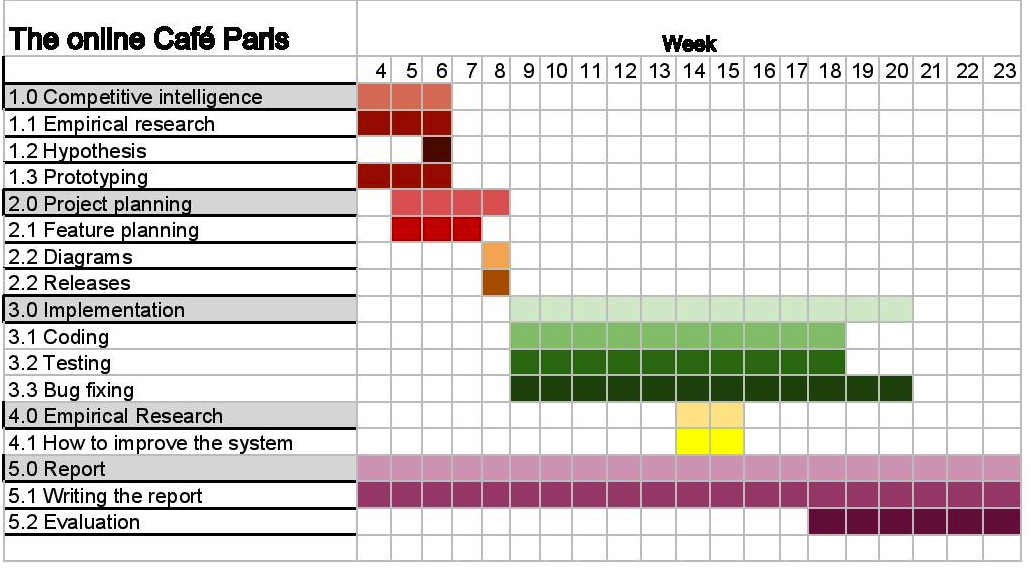
\includegraphics[width=0.8\textwidth,keepaspectratio]{grovplanering.jpg}
  \caption{A gantt-chart to guide us through the project and manage deadlines.}
\end{figure}
The work has been shared equally between the two participants in this project. All the planning, prestudy and implementing of the prototype was done together.

A huge part of project was new for us, we had no prior experience with WebGL, close to no experience in design and we had only written one application in javascript before. Because of this, and because we are only two people in the project, we decided not to have any specific roles. All the planning and research were done together and any important decision were discussed before implementing it. We tried to split the programming equally between the two of us, because both wanted to learn everything that was new to us. However, Patrik worked more on the backend and modifying Licode, while Alexandra had more focus on the design and additional features like paint and YouTube.
\subsection{What the site looks like}
These pictures will give you an idea of how the site is build up and it is easier to understand the idea, technologies, features and of course the design.
\subsubsection{Index/start page}
\begin{figure}[H]
  \centering
	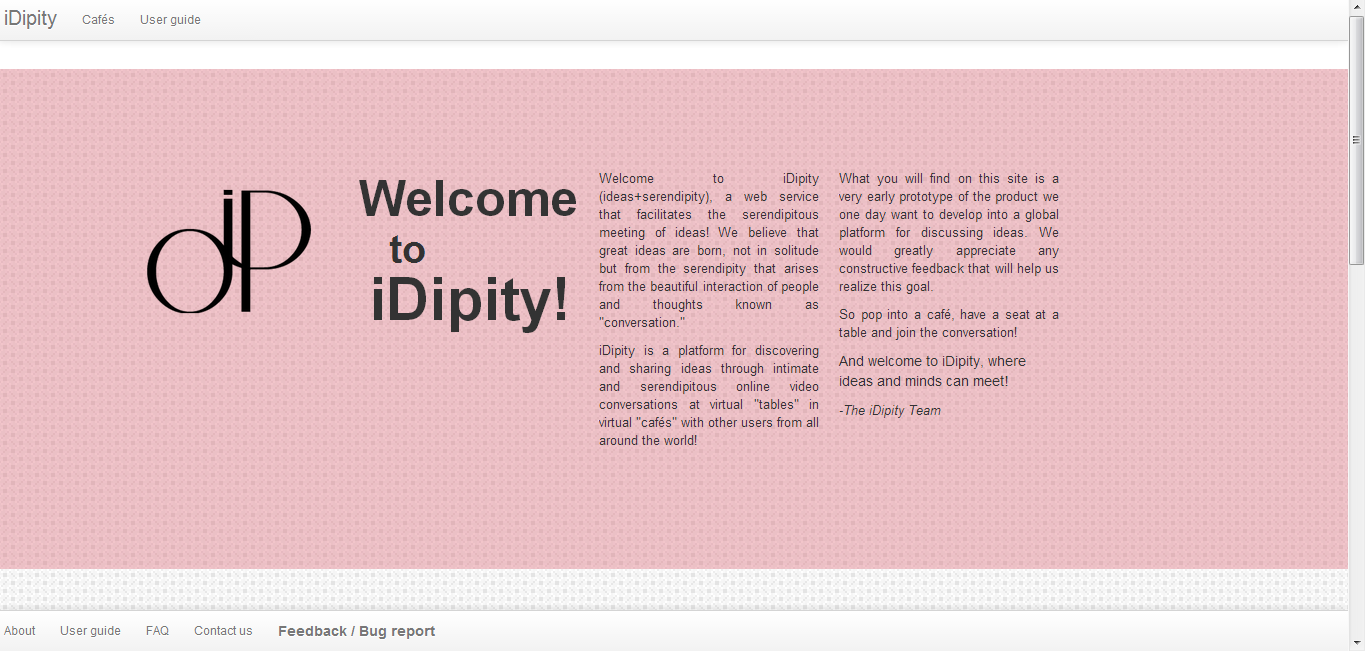
\includegraphics[width=0.8\textwidth,keepaspectratio]{indexpage1.png}
  \caption{The start page with a welcome message and some information about the site.}
\end{figure}
\begin{figure}[H]
  \centering
	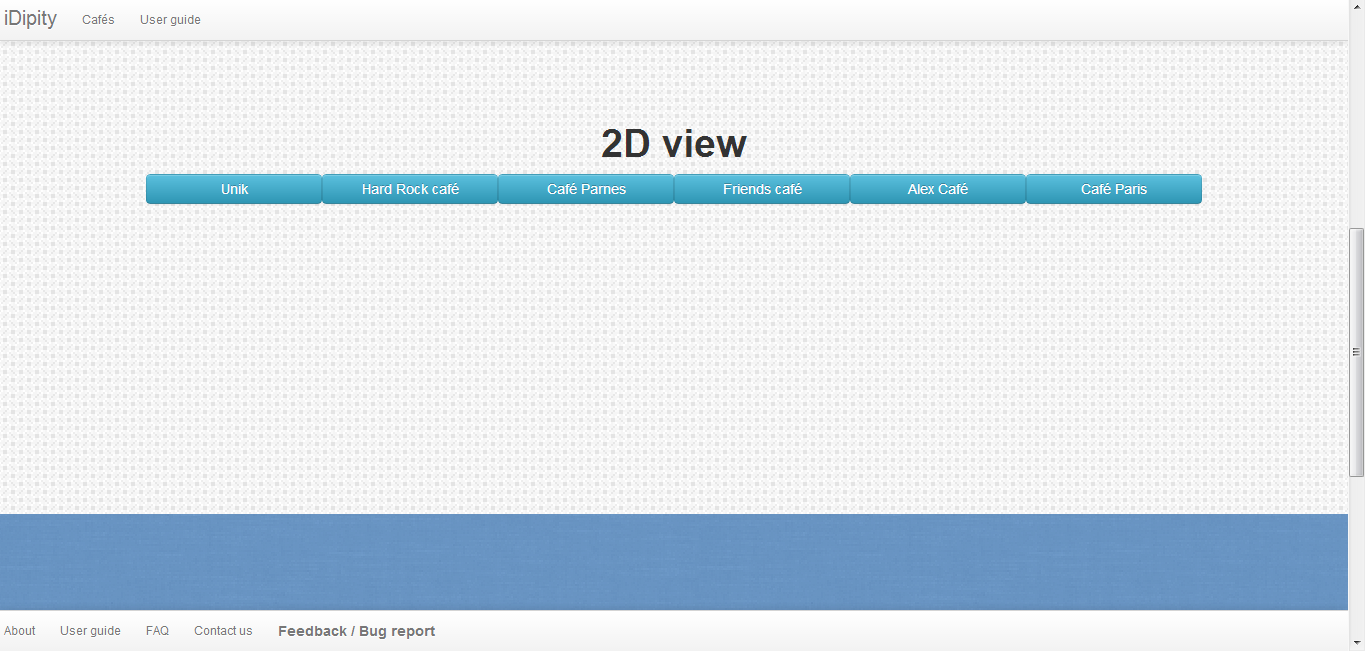
\includegraphics[width=0.8\textwidth,keepaspectratio]{indexpage2.png}
  \caption{The start page, the buttons are the six cafés the user can visit, this is the 2D view.}
\end{figure}
\begin{figure}[H]
  \centering
	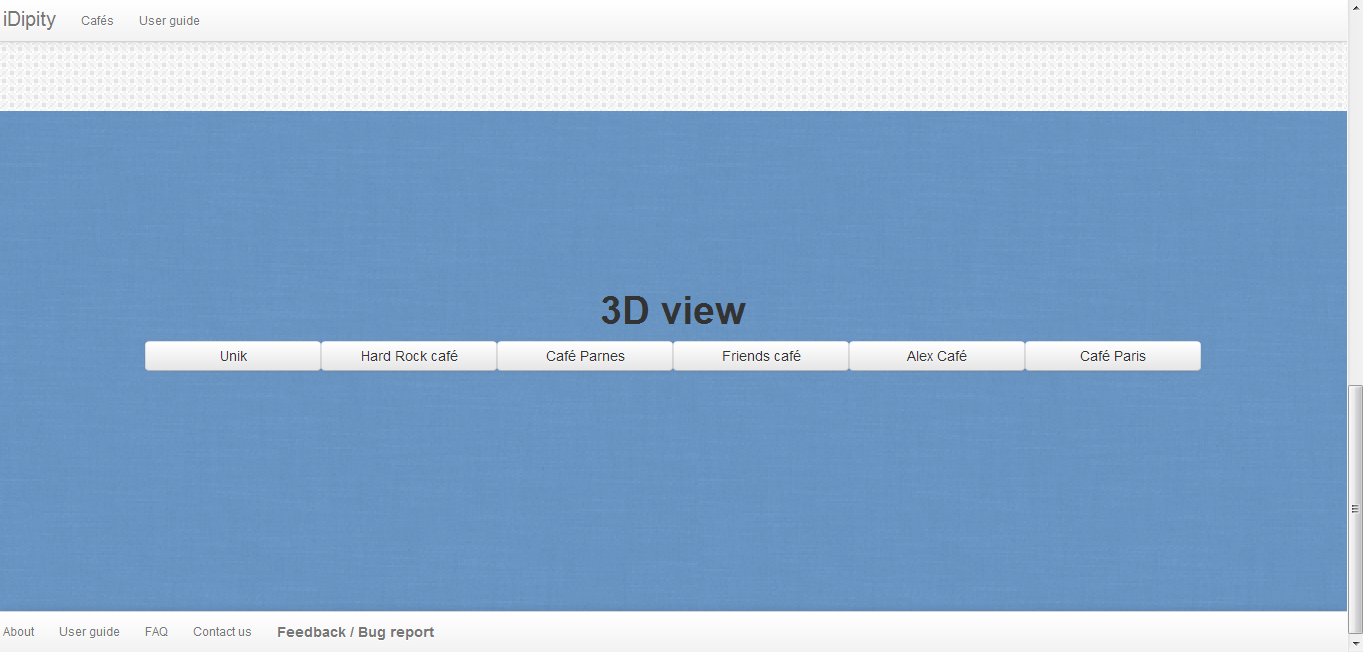
\includegraphics[width=0.8\textwidth,keepaspectratio]{indexpage3.png}
  \caption{The start page, the buttons are the six cafés the user can visit, this is the 3D view.}
\end{figure}
\subsubsection{Cafeview}
\begin{figure}[H]
  \centering
	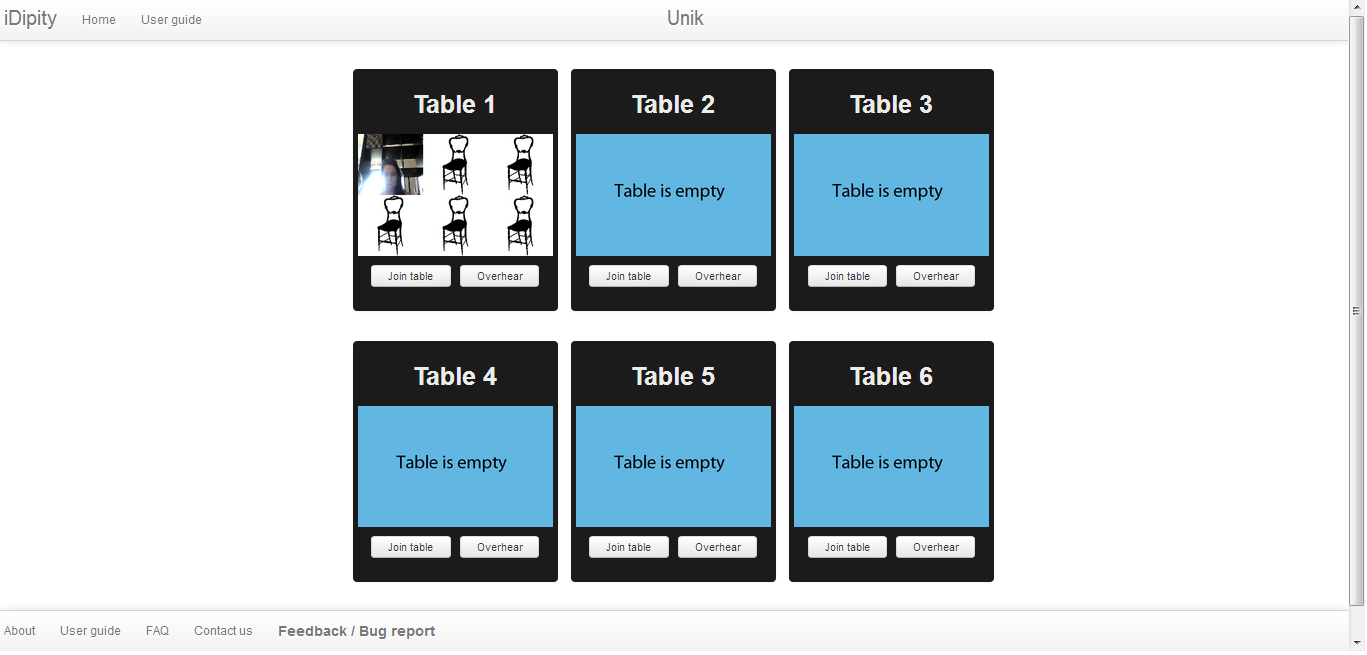
\includegraphics[width=0.8\textwidth,keepaspectratio]{thetables.png}
  \caption{This picture shows the tables in the café Unik. In table 1 there is one person sitting down, the other seats is empty at that table.}
\end{figure}
\begin{figure}[H]
  \centering
	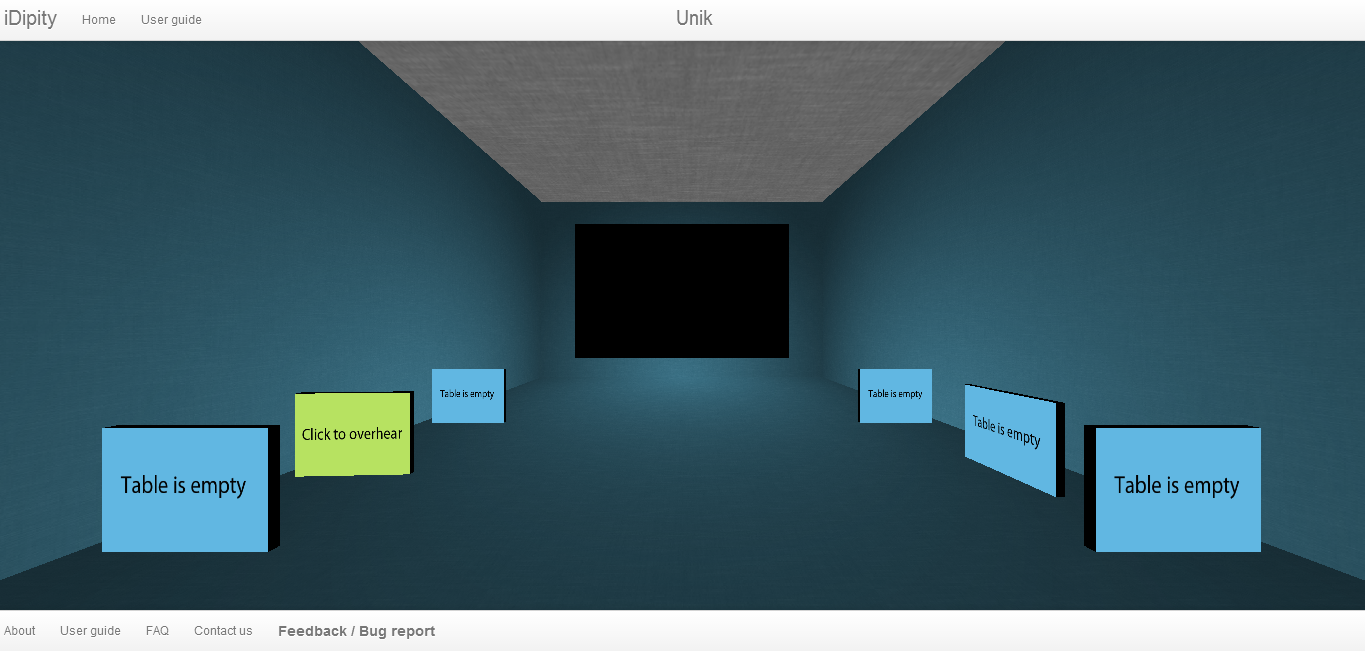
\includegraphics[width=0.8\textwidth,keepaspectratio]{thetables3D.png}
  \caption{This picture shows all the tables in café Unik. At the moment all the tables are empty. The green table is turned around with the mouse, if you click the on the turned table you will overhear the conversation if the table is not empty. If you click at a table you will sit down at the table.}
\end{figure}

\subsubsection{Tableview}
\begin{figure}[H]
  \centering
	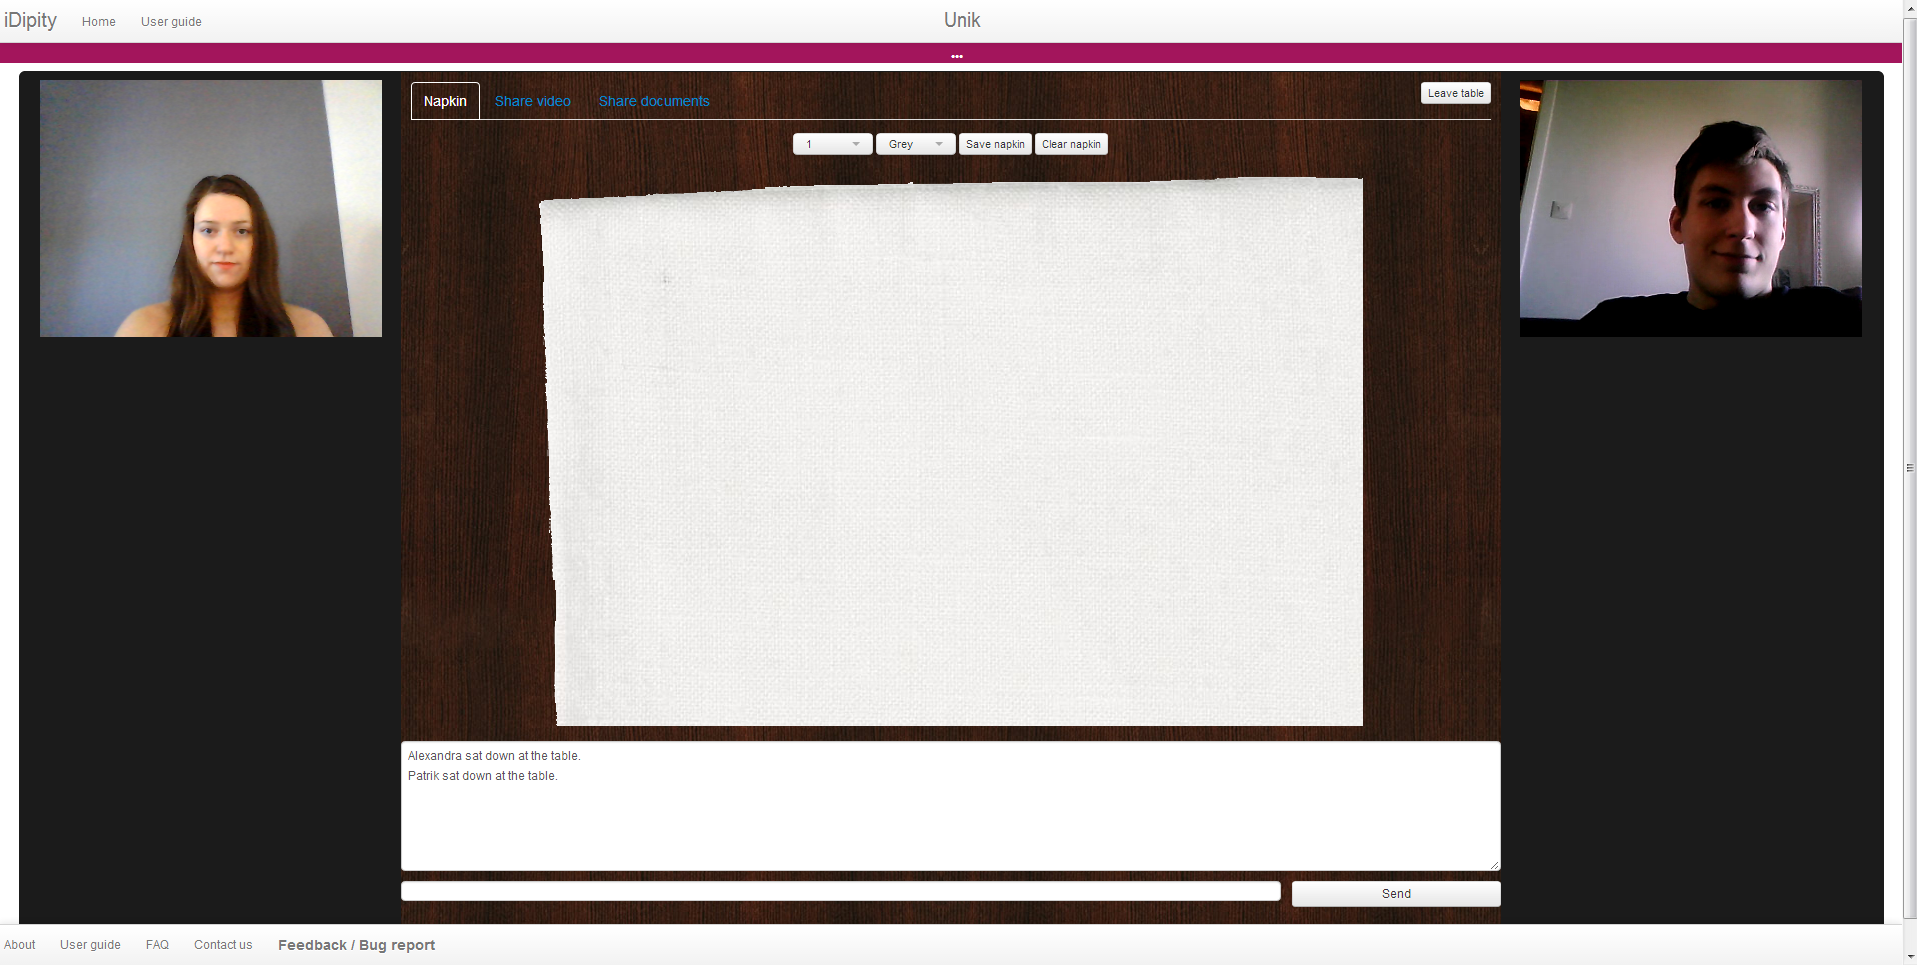
\includegraphics[width=0.8\textwidth,keepaspectratio]{sittingdown2D.png}
  \caption{This is how it looks like when you sitting down at a table having a video conversation with someone. You see the text chat and the napkin.}
\end{figure}
\begin{figure}[H]
  \centering
	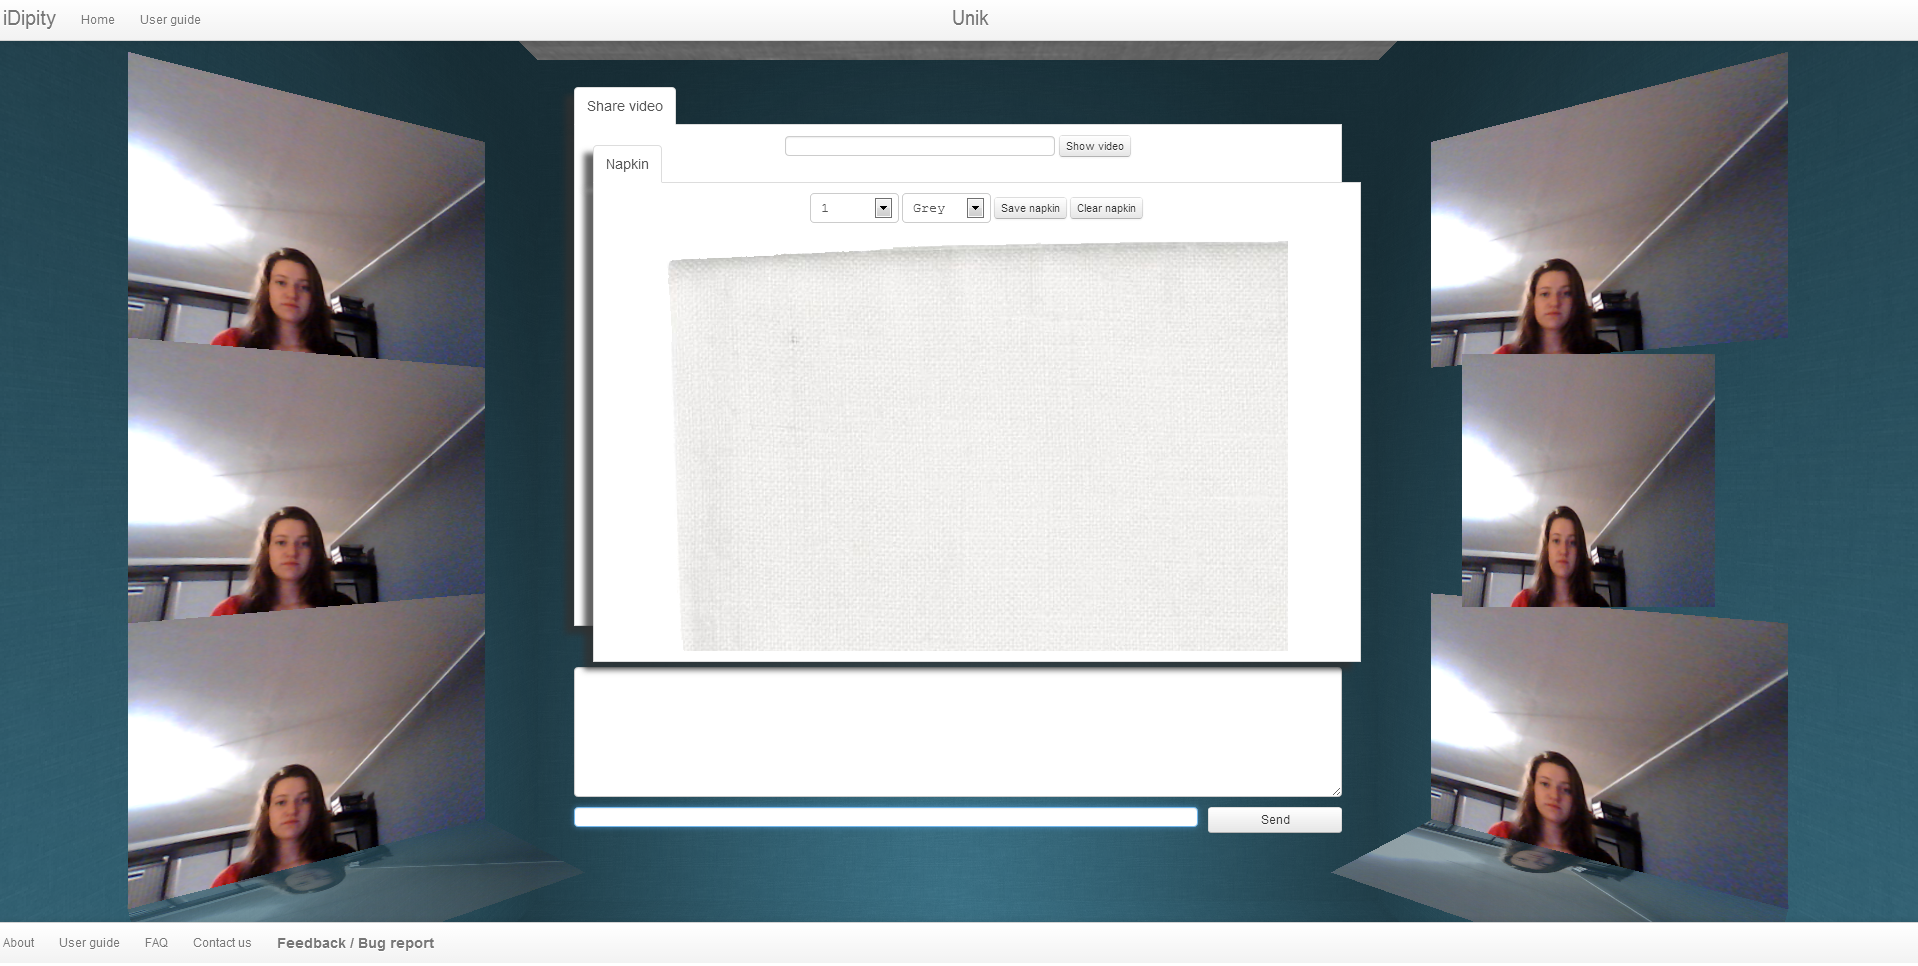
\includegraphics[width=0.8\textwidth,keepaspectratio]{sittingdown3D.png}
  \caption{This is how it looks like when you sitting down at a table having a video conversation with someone. You see the text chat and the napkin. The video stream in middle to the right has a mouse over it. That is why it looks different.}
\end{figure}
\subsection{Use cases}
These use cases are made for a better understanding of how the system can be used. Three example will explain this.
\subsubsection{Use case 1: Enter a café}
Lisa has a new idea for a product she wants to discuss. She starts her web browser and open Paris Café web page. She is met with a welcoming message and a list of the available cafés. After choosing a café she will be asked to enter her name into a form before continuing to the tables of the café. Once done she will be met by six “tables”. 
\subsubsection{Use case 2: Oversee and overhear}
When Lisa is inside a café she can look at the six tables. Each table will display an image of the persons, if any, sitting at the tables. When she has found a table that looks interesting she can choose to overhear and oversee the persons at the table by clicking the button “overhear”. The image will then be replaced by live video streams of the participants, including audio.
\subsubsection{Use case 3: Sit down at table}
After finding a table to sit down at she clicks “Join table”. Participants of the group will hear a knocking sound and find a notification in the upper right corner. They will now answer yes or no. If the majority answer yes she will sit down at a table where the video chat begins.
\section{Technologies}
\subsection{Node.js}
Node.js\cite{26} is an event-driven, non-blocking I/O JavaScript platform, built on Chrome's V8 JavaScript runtime. The reason for using Node.js is that it makes it easy to build fast and scalable network applications. The server is entirely written under the Node.js platform.
\subsection{WebRTC}
WebRTC\cite{27} (Web Real-Time Communication) enable browser to browser applications for voice calling, video chat and peer-to-peer file sharing without any plugins. A requirement for WebRTC is to use it in conjunction with HTML5. WebRTC is available in Chrome's stable version and in Firefox's Nightly version.

Using peer-to-peer connection instead of sending information through a central server removes the need for a powerful server. A server is still needed to setup the connection between the participants.
\subsection{Licode}
Licode\cite{28} is an open-source project that is based upon WebRTC technologies. It comes with Erizo, a Multipoint Control Unit(MCU) and an easy to use API for creating video conference rooms directly in the browser. 
\subsubsection{Erizo}
Erizo is an MCU written in C++. It's fully compatible with WebRTC standards and protocols. Erizo does not currently provide any transcoding of videos but it's being worked on right now. 
\subsubsection{Nuve}
Nuve makes it possible to create and manage video conference rooms. It holds information about each room and let's you ask for example a user list. It is designed to scale on the cloud.
\subsection{MongoDB}
MongoDB\cite{29} is an open-source, document-oriented database designed for ease of development and scaling. Stores data as JSON-like documents dynamically and making the integration of data and our prototype easier and faster.
\subsection{Mongoose}
Mongoose\cite{30} is an object data modeling library for MongoDB. It allows you to create models for your data, creating a structure to MongoDB while maintaining it's flexibility.
\subsection{Express}
Express\cite{31} is a fast and small node.js web application framework, providing a powerful routing system which allows you to easily create single and multi-page web applications. It helps you manage everything, from routes, to handling requests and views.
\subsection{Twitter Bootstrap}
Twitter Bootstrap\cite{32}is a collection of tools for creating beautiful web applications without being an expert on design. It includes HTML, JS and CSS-based design templates for typography, forms, buttons, charts, navigation and other interface components. The reason for using Twitter Bootstrap is to get a nice interface and it is easy to use.
\subsection{HTML5}
HTML is used to structure and presents information on a website, HTML5 is the newest HTML standard. It's designed to make web programming easier and more interactive. Some of the new features that are interesting for our project is the <video> and <canvas> elements.
\subsection{Three.js}
Three.js\cite{33} is a lightweight cross-browser JavaScript library/API used to create and display animated 3D computer graphics on a Web browser. Three.js scripts may be used in conjunction with the HTML5 canvas element, SVG or WebGL. We decided to go with WebGL.
\subsubsection{WebGL}
WebGL (Web Graphics Library) is a JavaScript API that allows the client to render powerful 3D graphics within the browser without plugins. It runs on computers GPU.

Our purpose of using WebGL is to try the café Paris website with a virtual 3D environment. This makes us a good case to try out a mixed reality, by combining a virtual 3D environment with the users video stream we can transfer the feeling of actually being in a real café into our website. Overseeing, overhearing and mingling
\subsection{GitHub}
For revision control and code management we use Git. Git is a open source distributed revision control system. To simplify the setup we chose to host the repository at Github\cite{34}.

\section{Method}
Some information was collected before implementing the service. A study was made in order to find suitable ways of overhearing, overseeing and mingle. And a comparison of different WebRTC frameworks was necessary for us due to the video conference features.
\subsection{WebRTC comparison}
WebRTC is a new web standard for peer-to-peer communication. WebRTC allow browsers to send information to each other, without going through a server. The focus is currently on audio and video communication but they will implement a data channel in the future. This will drastically decrease the server load.

We compared many different WebRTC framework before settling with Licode. Licode offered something that others didn't, and something that is necessary if the system would be used on a larger scale. That feature is a Multipoint Control Unit(MCU). Here follows a short summary of the runner ups.
\subsubsection{Easy RTC}
EasyRTC is an open source WebRTC framework with cross browser support. It allows you to easily steup a Node.js server and provides an API for making advanced web applications in no time. EasyRTC uses websockets for fast message passing between clients.
\subsubsection{WebRTC.io}
WebRTC.io aims to make it easier to use the new webstandard. It does this by providing a simple abstraction layer for the otherwise semi-low level WebRTC.
\subsubsection{Holla}
Holla is another abstraction layer with the same goal, to make it easier to work with WebRTC. Holla provides a client and a Node.js server module. The server is used to initiate the communication between the clients. Each client registers a username that is used for making calls or sending data to each other.
\subsection{Survey}
A survey was made during the early stages of the project. The idea was to get a grasp of how people feel about visiting a virtual café online as well as to capture their opinion on what aspects of a real café makes it such a good place for intimate discussions.
\subsubsection{Evaluation}
The most important aspects of a café is the intimate environment and the other people in the café. This means that in order for us to capture that intimate feeling of a café, we have to create a design that gives a similar feeling

The result showed that people like the ability to overhear other conversations going on in the café. But it also showed that it can be a disturbing factor when you can't block out the noise.

Mingle is big part of the master thesis. How can you ask to participate in a conversation without disturbing the group of people having the conversation. The answers shows that a subtle knock or a short personal message to the group would get their attention without drawing them away from the conversation.

We had a few questions concerning a 3D environment. The answers however were pretty much evenly distributed between “yes” and “no” and due to the amount of participants we can't see any clear result. However, we believe that it can be hard to imagine going to a café in a 3D virtual environment and that a new survey when we have a prototype running would result in different answers.
\subsection{Prestudy conclusion}
After doing this research we have noticed the huge amount of different video conferencing systems each with their own solution for specific problems. All from high-end systems designed for big businesses, to small systems for personal use.

The result however, strongly motivates our research questions. While there exists a few good services for video conference and online group collaboration the only ones that support multiple groups is within a 3D environment and not one of these have strong focus on mingling.

There is still room for improvements in overhearing and mingling, both inside and outside a 3D environment.

If using virtual 3D environments, a mixed reality is interesting for us to mix real peoples video stream with an virtual environment. If a person who has joined a conversation at a table does not want to share his video stream he may just get an avatar to represent him instead a video stream. It would also make it possible to enable human expressions and gestures[9].
\subsection{System architecture}
The system consists of two different parts, the backend and the frontend.
\begin{figure}[H]
  \centering
	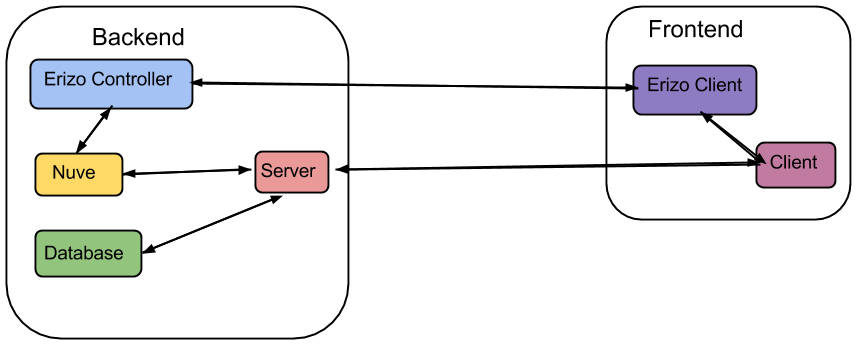
\includegraphics[width=0.8\textwidth,keepaspectratio]{systemarchitecture.png}
  \caption{A chart over the system architecture.}
\end{figure}
\subsubsection{Backend}
The main part is the Node.js server. The server acts like a middleman for the Licode modules and the frontend. It communicates with the clients using standard HTTP requests and a simple RESTful API together with Express.js. It allows the client to easily GET/POST data from/to the server. The server also communicates with Nuve via a token based communication mechanism.

Example: GET /api/getCafe/Unik from the database results in:
%{
"name": "Unik",
"table1": "513dd08a07aa2f143700001f",
"table2": "513dd08b07aa2f1437000020",
"table3": "513dd08c07aa2f1437000021",
"table4": "513dd08d07aa2f1437000022",
"table5": "513dd08e07aa2f1437000023",
"table6": "513dd08f07aa2f1437000024"
%}
\subsubsection{Database}
The database stores all the information about the cafés, all the rooms and what rooms that belongs to what café and the snapshot taken by all leaders in each room. Each café consists of six rooms. The client communicates with the server in which the server communicated with the database.
\subsubsection{Server}
All the cafés and rooms are created in the server using Nuve Client. An access request will be sent and accepted via Nuve for each user trying to connect to a room via a token-based authentication mechanism. This mechanism allows the server to create access tokens, and it will provide these tokens to the clients. 
\subsubsection{Nuve}
Nuve is a Licode module that manages the rooms or the tokens to access to a determined room. Nuve Client API allows the server to, for example, create rooms, get rooms, and get users of a certain room.
\subsubsection{Erizo Controller}
Erizo controller communicates with Erizo. It handles the subscription of streams, sends the streams to all subscribers and controls the rooms. Erizo controller scales well and spawns new instances when the pressure is high.
\subsubsection{Frontend}
The frontend is built using HTML5, JQuery, Javascript and Erizo. The frontend communicates with two different parts of the system. It speaks to the server for HTML/CSS/JS files, tokens and database access. All the communication between different clients goes through Erizo controller. This means that all the data (Audio, Video or data) from a stream is sent to Erizo controller and then forwarded to all the client who subscribes to said stream.
\subsubsection{Erizo Client}
Erizo client provides a javascript API for communicating with Erizo Controller. It allows the client to, for example, publish and subscribe streams, create video elements
\subsection{Setting up a connection}
The client requests a token from the server which in turn ask Nuve. The token includes an ip-address to Erizo Controller. When you connect to a room the client establishes a websocket connection with Erizo Controller. When you publish your own stream or subscribe to other streams the web client exchanges Session Description Protocol messages with Erizo Controller in order to negotiate media type, format and all associated properties. When the negotiation is done the client and Erizo Controller establish a Secure Real-time Transport Protocol connection to deliver audio and video.
\section{Result}
Here follows the result of the main features and different pages on the website.
\subsection{Design}
The design is an important feature of the system. In order to capture the feeling of being in a cafe, we need to create a modern design that is just as intimate as a real life café. The design is mostly done using Twitter Bootstrap. Bootstrap helped attaining a clean and modern look. A few goals was set up for the design, one was that the site would look just as good and work just as well on big and small resolutions. Therefore, percentage were used on almost all sizes so everything keeps the aspect ratio when the window is resized. 

Another goal was the site navigation. It should be self-explanatory, easy to navigate and accessible in a few clicks.
\subsubsection{The 2D view}
The website has three important pages, index, cafeview and table view.

When the user first enters the site they will see a welcoming message, explaining the purpose of the site. If they scroll down they will see a list of café buttons for each of the view type, 2D and 3D. On the top bar is a link to a user guide and on the bottom a link to send us a feedback mail.

The Cafeview is after you have entered a café. It displays the tables of the café and an image of the participants of each table. The user can chose to sit down at a table or overhear the table by pressing respective button.

The Tableview consists of 2 parts. There is what we call a table in the middle of the page, with room for 3 streams on each side. We chose to limit the number of participants in each room to six. There are tabs on the top side of the table. These are filled with features for the users. While video chatting, the users can draw, watch a YouTube clip and chat together. 
\subsubsection{The 3D view}
The first idea was to create an environment with the feeling of being in a real café, a room with tables, the video streams in the room of all the participants and also you can walk around in the café to see all the tables. After our market research we found out that this type of environment was not desirable and also we think that we can reach a bigger audience by avoiding it. We decided to reuse the 2D view and represent it in a 3D view to enhance the feeling of being in the same room. 

The Caféview has been completely remade. When you enter a cafe you will see a large room with blocks that represents tables. These blocks are rotatable. You will also see a big screen on the wall, after rotating a block and clicking on the backside,  the live video streams will show on that screen.

The Tableview has been improved in many ways. The video streams are slightly rotated towards the center of the screen. This gives the feeling of sitting around a table with your friends. The background has been given depth in order to give the feeling of being in a room. The tabs with the napkin and share YouTube video is now in different layers. They will switch places when you click on them.
\subsection{Leader}
Each room needs its own leader to enable some features below. If a room is empty when someone enter, he or she is automatically chosen to be the leader in that room. A new leader will be chosen if the current leader leaves the room, this is done by letting each user ping the server 3 times. The one with the lowest mean value becomes the leader. By doing this we know the leader will have the lowest latency of the group. If two or more users have the same mean value, the one with the highest stream ID becomes the leader.

By letting the leader take care of some of the features instead of letting the server handle it, we reduce the server load. The server does not even know about what the leader is up to due to the peer-to-peer connection.
\subsection{Peer-to-peer}
WebRTC allows data to be sent between the clients using peer-to-peer. We chose to take advantage of this feature in order to release some stress from the server. The media and data streams are separated in order to create a simple messaging service that can be used by all features on the site, to communicate between the clients without the server.
\subsection{Overhearing}
You can only block out noise to some extent in a real environment. However, in a virtual environment we can chose when and what to overhear. Just like you can focus your hearing to a certain point we can chose to listen to a certain table.

The audio can not be separated from the video and because of that we chose to display video as well when you overhear a table. When you press the overhearing button, you will subscribe to all the streams at the table without publishing your own stream. The snapshot image for the table will be replaced with live video streams. This means you can hear and see the group without them being able to see or hear you. When the user choses to end the overhearing, the streams will be removed and replaced with the snapshot image.
\begin{figure}[H]
  \centering
	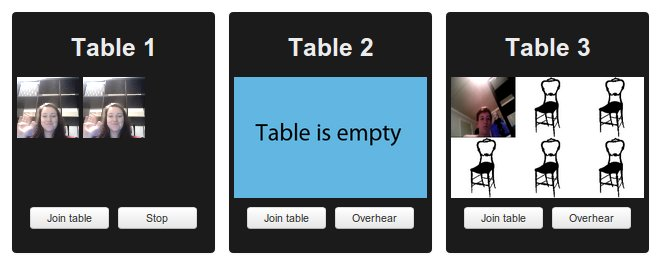
\includegraphics[width=0.8\textwidth,keepaspectratio]{overhear2d.jpg}
  \caption{Real-time overseeing and overhearing in the 2D view.}
\end{figure}
\begin{figure}[H]
  \centering
	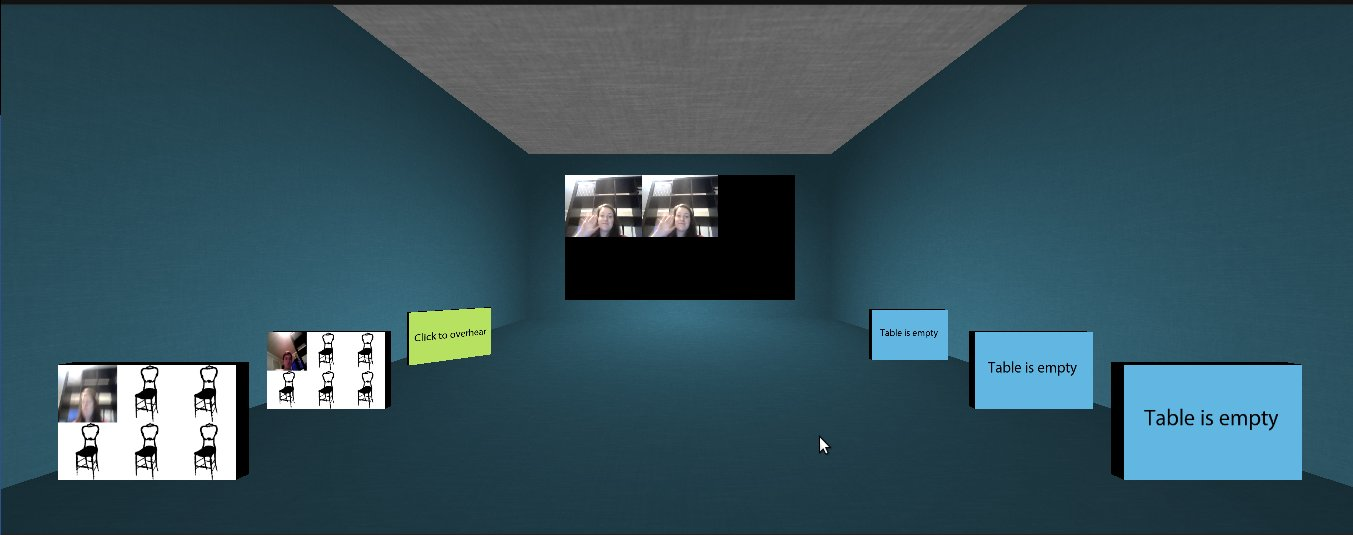
\includegraphics[width=0.8\textwidth,keepaspectratio]{3doverhearing.jpg}
  \caption{Real-time overseeing and overhearing in the 3D view.}
\end{figure}
We chose to not display the text chat, drawing or if a video is watched. This is meant to give the users a bit of privacy. 

We chose not to implement overhearing when you're in a table. This is because it would draw attention from the conversation.

\subsection{Overseeing}
The prototype has three kinds of overseeing. The first one is directly when you enter the café. You then see a snapshot of every stream for every table in the café[Figure 12]. The snapshots updates every 30 seconds, when a new user sits down at a table and when a user leaves a table. The snapshot is sent to the server by a chosen leader of each table.
\begin{figure}[H]
  \centering
	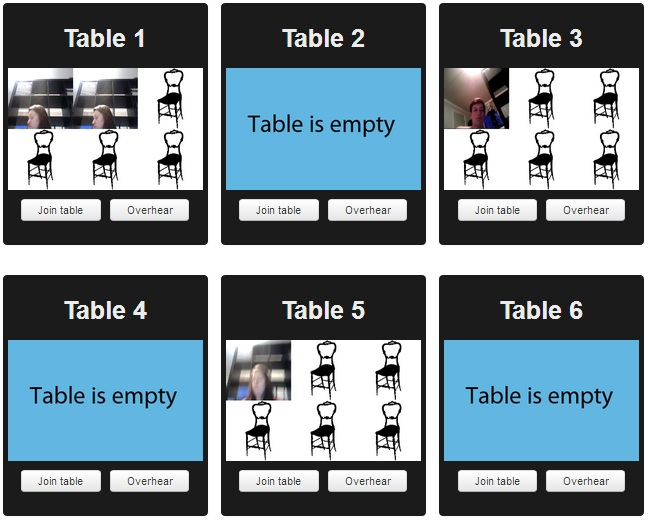
\includegraphics[width=0.8\textwidth,keepaspectratio]{overseeing2D.jpg}
  \caption{Shows overseeing when you enter a café and view the tables.}
\end{figure}
The second type of overseeing is in real-time. Before you sit down at a table you can chose to oversee and overhear the by clicking a button. You can then see and hear all the participants at the table in real-time[Figure 10, 11].

The third type of overseeing is when you are in a room sitting down at a table. In a real café you can actually look around the café and see the other participant while still have a conversation with your table, we decided to implement this by having a bar on the top of the page that you can pull down[Figure 13] to see the snapshots of the other tables in the same café you are in.
\begin{figure}[H]
  \centering
	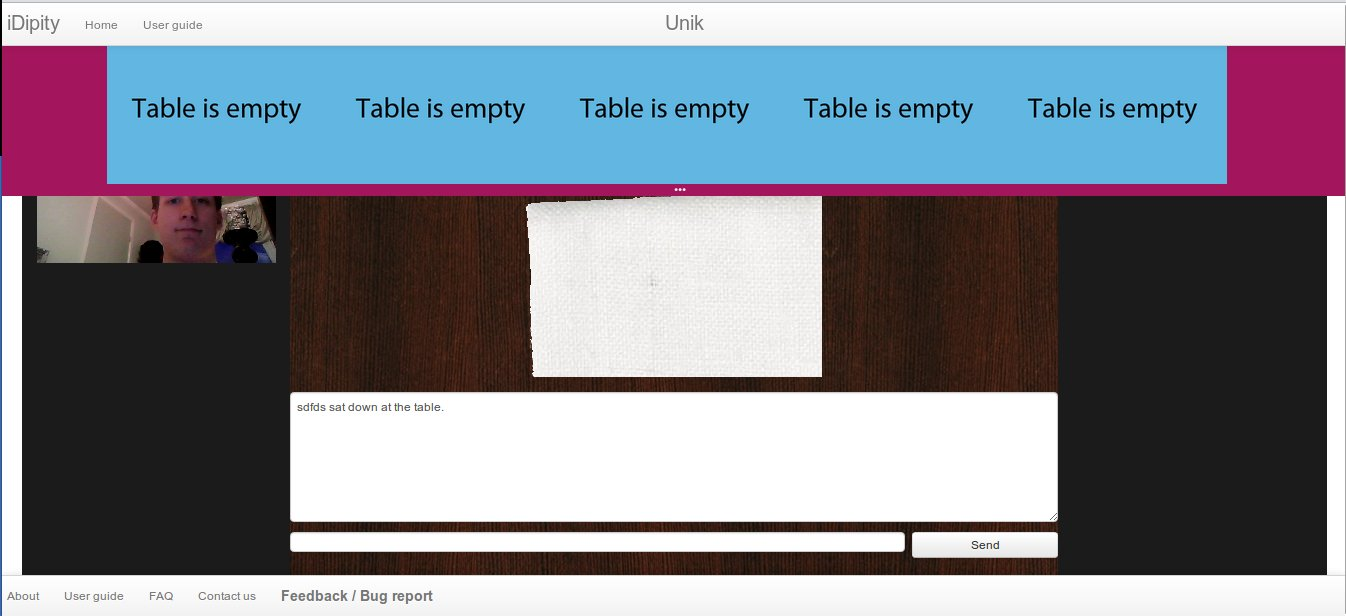
\includegraphics[width=0.8\textwidth,keepaspectratio]{pulldownoversee.jpg}
  \caption{Pulldown overseeing from inside a café. Displays the snapshot images of the other tables in the café.}
\end{figure}
To enable overseeing on the website the leader takes a snapshot of every user in the room as mentioned above. The client will then encode the binary data from the image to a base64 string and send it to the server. The server will then store the string in the database.

To see all the snapshots in the Cafeview the client sends an HTTP request to the server and gets a JSON-object in response.
\subsection{Mingle}
The idea was to have a subtle way of telling the participants at a certain table you want to sit down and join the conversation. We had many ideas for how this could be realised, for example a personal text message to the group, record a voice message or just a simple knock. After the study we decided to go with the knock because reading a text message or listening to a voice message would take the focus away from the conversation. 
\begin{figure}[H]
  \centering
	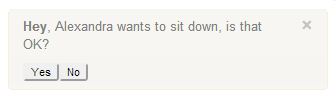
\includegraphics[width=0.8\textwidth,keepaspectratio]{knock.png}
  \caption{A knock notification. Alexandra wants to join the room.}
\end{figure}
After pressing the knock button, a datastream is published and other datastreams are being subscribed to. A message is sent to all the users in the room and a notification[Figure 14] pops up in the upper right corner. All the users in the room gets to vote by pressing “Yes” or “No”. The notification disappears after 20 seconds. Any unanswered notification results in a “No” The answers are sent to the requesters client and depending on how many “Yes”, you have to have more than the total amount of users in the room divided by two plus one, so the majority has to answer “Yes” before a user can connect to the room and publish his or her media stream.

To again save some server load the knocking is done with peer-to-peer connection, means that the server does not have a clue of who is knocking and it is all done between the clients involved.
\subsection{Paint}
Many ideas starts on a napkin, maybe in a café just hanging with your colleagues or friends. The napkin at the table is shared between all the users sitting at the same table and they can all draw on it together[Figure 15], real-time collaboration. When a new user sits down at the table he or she will get the current napkin by each tables leader. The napkin can also be saved locally to your computer. The clear napkin button will reset the napkin for all users. Color and thickness can be chosen in the dropdown menus.
\begin{figure}[H]
  \centering
	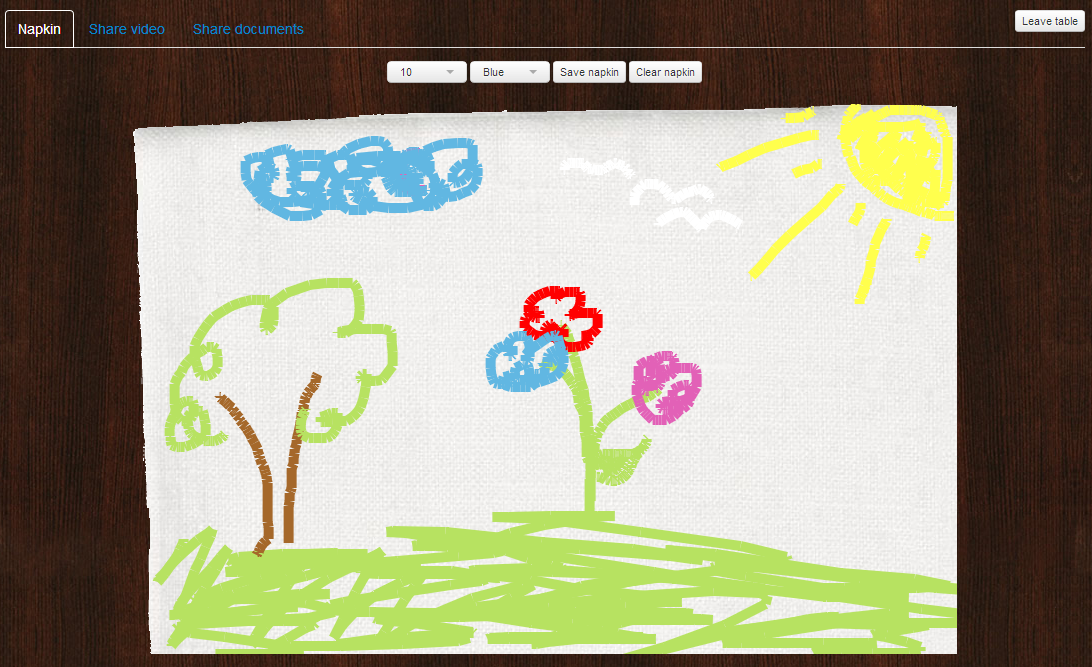
\includegraphics[width=0.8\textwidth,keepaspectratio]{theNapkin.png}
  \caption{A drawing on the napkin shared with all participants in the room.}
\end{figure}
\subsection{YouTube}
A synchronized YouTube player that plays any video from YouTube[Figure 16]. To play a video you paste an URL into a field and it will be shared amongst the group. Pressing play or pause will play and pause the video for all participants in the room. If you decides to close the video it will only close for you and the rest of the group can still watch the video together.
\begin{figure}[H]
  \centering
	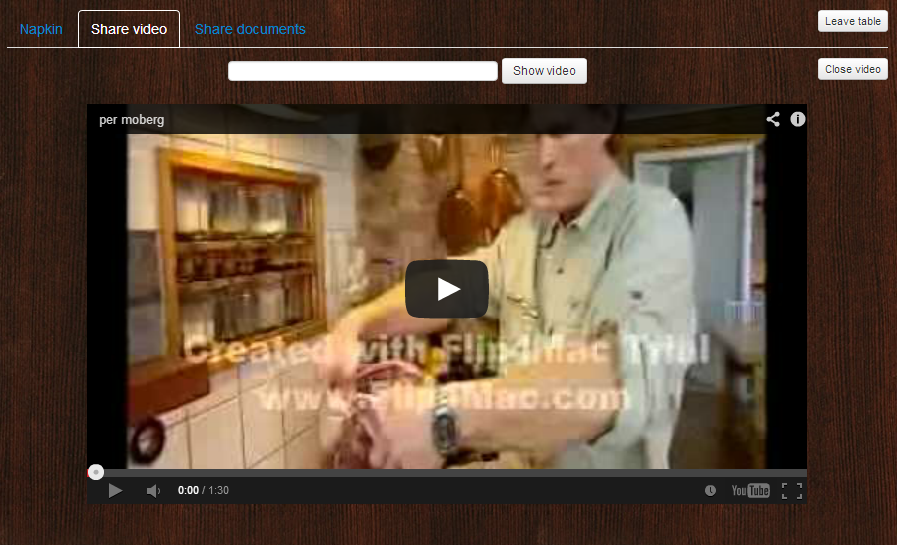
\includegraphics[width=0.8\textwidth,keepaspectratio]{youtubeToReport.png}
  \caption{The youtube player in the 2D view.}
\end{figure}
\subsection{Text chat}
The text chat is very basic[Figure 17]. You chose a username when you enter a café. This will be displayed whenever you write a message in the chat. The chat is also used for some notifications, for example when someone sits down at a table. All the text messages is shared with all participants at the table.
\begin{figure}[H]
  \centering
	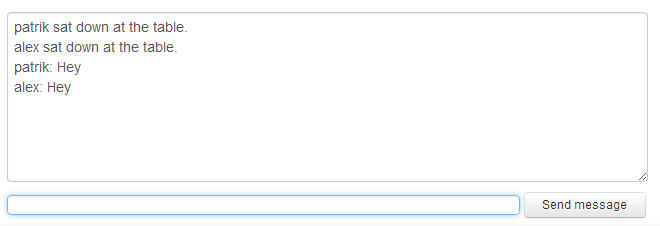
\includegraphics[width=0.8\textwidth,keepaspectratio]{chat.png}
  \caption{A knock notification. Alexandra wants to join the room.}
\end{figure}
\subsection{Server performance}
The reason for using an MCU is to reduce the required bandwidth for every client. This means that more people with not as good bandwidth can still use the service even if they don't have very high bandwidth. 

Using peer-to-peer would mean that every user sends his or her stream to every other user in the room, as well as to everyone that is overhearing. Instead by using an MCU, each user sends a stream to the MCU, Erizo. Erizo then perform some basic transcoding, if any, before forwarding the data to each other user in the same room, as well as to everyone who is overhearing.

%Table
\subsubsection{Theory}
To understand the importance of an MCU, we will now compare the required bandwidth on both server and client, with and without the MCU.
\paragraph{Without MCU.}
Scenario: A room with 6 users and 2 people overhearing and overseeing in real-time.

Let U denote amount of users in a room, O the amount of users overhearing a certain room and S the bandwidth of a stream. 

Each client then send his or her stream to each other client in the room, plus each overhearing client.
\\*
\\*
The data sent from each client is then $S*(U-1)+S*O$\\*
The data received at each client is $S*(U-1)$\\*
The data received at each overhearing client is $S*U$\\*
The data sent from and to the server is close to zero and will not be counted.
\\*\\*
Let's say each stream has a bandwidth of 200 KB/s and calculate the above scenario.
\\*
\\*
$200*5 + 200*3 = 1600$ KB/s $= 12.8$ Mbps sent from each client in the room\\*
$200*5 = 1000$ KB/S  $= 8$ Mbps sent to each client in the room\\*
$200*6 = 1200$ KB/s $= 9.6$ Mbps sent to each overhearing client\\*

The calculations show that for a client to work with our service with streams of $200$ KB/s, it needs a bandwidth of atleast 8 Mbit downstream and atleast 8 Mbit upstream. And this is without anyone overhearing. This is very high bandwidth requirements for one person and service and it also would not work on a larger scale if some table gets too many people overhearing at the same time. If the system instead had a MCU it would not matter which table got overheard since the total amount of data sent from the server would not change depending on if five people are overhearing the same table or five different tables.
\paragraph{With MCU.}
So same scenario again, this time with the MCU. All clients will now send their stream to the MCU, which forwards it to all subscribers.
\\*
\\*
The data sent from the server is $U((U-1)*S) + O*U*S$.\\* 
The date sent to the server is $U*S$.\\*
The data received at each client is $S*(U-1)$.\\*
The data received at each overhearing client is $S*U$.\\*

An example. If we have one room with 6 users and 3 people overhearing with a bitrate of $200$ KB/s results in:

$6*200 = 1 200$ KB/s $= 9.6$ Mbps sent to the server.
$6*(5*200) + 3*6*200 = 9 600$ KB/s = $76.80$ Mbps sent from the server.
$200*5 = 1000$ KB/S  $= 8$ Mbps sent to each client in the room
$200*6 = 1200$ KB/s $= 9.6$ Mbps sent to each overhearing client

Now let's assume we have a server with a dedicated 1Gbit connection.

1Gbit $= 131 072$ KB.
The bandwidth needed to fill a room without overhearing is $6*(5*200) = 6 000 KB/s$
$131 072/6 000 = 21.8453333333$. So a 1Gbit connection can manage almost 22 filled rooms at a time. However, we need to keep in mind that $200$ KB/s equals to over 1.5 Mbps. In comparison, Skype recommends 500 kbps bandwidth for high quality video[25].
\subsubsection{Performance test}

A performance test was done in order to see how the system would perform under pressure and to get a feeling of the hardware requirements on a larger scale. 4 computers including the server were used during the test.
\begin{center}
    \begin{tabular}{| l | l | l | l | l |}
    \hline
    Device & OS & Processor & Ram \\ \hline
    iMac & Mac OS X & Intel Core i5 3.1 GHz & 16 GB\\ \hline
    Asus Laptop & Windows 7 & Intel Core i7 2.2 GHz & 8 GB \\ \hline
    Mac mini & Mac OS X & Intel Core i7 2.7 GHz & 4 GB \\ \hline
    Server & Ubuntu 12.10 & Intel Xeon i5 2.4 GHz & 2 GB\\ \hline
    \end{tabular}
\end{center}
As we saw from the theory, the bottleneck lies in data sent from the server. The CPU usage peaked at a bit over 50\% while the video quality of the streams lowered because the server couldn't send out more than 4 MB/s.

The result of the test followed the theory closely, as you can see in the table.

\begin{center}
    \begin{tabular}{| l | l | l | l |}
    \hline
    Streams(Nr) & Incoming data(KB/s) & Outgoing data(KB/s) & Comment \\ \hline
    1 & 45 & 0 & \\ \hline
    2 & 250 & 500 & \\ \hline
    3 & 800 & 1600 & \\ \hline
    4 & 1000 & 3200 &\\ \hline
    4 & 1000 & 4000 &\\ \hline
    4 & 800 & 4000 & Lower video quality\\ \hline
    \end{tabular}
\end{center}

The video quality then continued to decrease for every new stream published or subscribed. We believe that once Licode start transcode/mixing the streams, the data sent from the server will be reduced and CPU usage increased. 
\section{Discussion}
During this project we discovered problems with some features and perhaps a way of solving some of them. All possible solutions will be presented here. Along with that discussions we also present feedback from test users.
\subsection{Issues}
We have one issue with the knocking function. If five people having a conversation at a table and two more people wants to join their conversation at the same time, if they both is accepted by the group they will both connect to the table. This only happens if they are trying to connect exactly at the same time, otherwise they will get rejected because we have a limit of maximum six users at once in one table. The time it takes for a user to connect to the table is the problem, the latest user will not get notified that he or she was too late. 
\subsection{The design}
We had almost no experience of web design and WebGL before starting this project. Here follows some improvements we think could be done to enhance the user experience.
\begin{itemize}
\item We have blocks representing tables in the 3D version of Cafeview. These could be exchanged with models of a table. 
\item It would be cool to have models of a person around the tables and map the video stream or snapshots to the face of the model.
\item Furnish the 3D Cafeview with perhaps bar, paintings and such, to make it look like like a real room.
\end{itemize}
\subsection{User test}
We collected a group of people to test our prototype in an attempt to get answers on our research questions. The test begun with that everybody entered the same café and the same table, all the features were tested, a drawing was made, we watched a YouTube video together and sending text messages to each other. After a time of playing around we sent them out of the room, one by one, to try the features outside the table, in the overview of all tables, overseeing and overhearing. We also tested overseeing when sitting at a table.

After the whole group tested all the features, they answered a questionnaire based on our research question.

The group found the snapshot images very practical and a good way to display the visitors or the café. They also liked being able to "look around" at the other tables while sitting at a table of their own. The overhearing part seems to have been a nice experience but they felt a bit freaky when listening to and seeing another conversation while not being a part of it. But they also said they would probably feel more comfortable overseeing and overhearing other people after using the service for a while.

People generally like the knocking because it was a good way see who wants to sit down at the table. However, they would like some more information about the person before deciding if he or she can join the conversation, for example a personal text message or being to check a user profile.

There were mixed feelings about having other people overhearing the conversation. Some thought it was exciting and a bit scary, others didn't even think about it. The group agreed on that the content of the conversation changes when they know other can be listening in on the conversation. That you have to think about what you say, just like in public places.

\subsection{Performance test}
The test result showed that the system is really heavy on the bandwidth. The MCU helps a lot by taking the stress away from the clients and making it easier for us to decide on a minimum bandwidth requirement. But it's not needed as much when there are few people in a room with no one overhearing. In fact, if there are only two people in the room both alternatives uses as much bandwidth, but a peer-to-peer connection would send the stream directly to each other resulting in less stress on the server without increasing the load on the clients.

So we see that we need an MCU in order for the service to work well with a large amount of clients. But the problem is still the bandwidth requirement and we see two solutions to this problem. The first one is to transcode the streams. This would increase the CPU load but drastically decrease the data sent from the server. The second solution is to limit the bitrate of the streams. The video quality as it is now is really high and limiting it to maybe 125 KB/s would drastically increase the maximum number of users on the system.
\subsection{Future work and improvements}
We set out to build a prototype that includes overseeing, overhearing and mingle, and that's what we have done. But this is a project done in limited time so there are of course plenty of ways to improve the system.

We wanted to activate overhearing by simply holding the mouse over a table. We tried it and it worked, but it was far from optimal. Connecting to a room and subscribing to a stream actually takes some time to do. And holding the mouse over a table for all that time is simply not something you want to do. A solution to this problem would be to first connect directly to the other users while waiting for Erizo to connect and then switch over to Erizo when it's done. This would drastically decrease the time required to hover before you start overhearing the users in the room.

To get the feeling that you actually having a conversation face to face with a person online in a video conference, the eyes and body gestures is important. In the related work part we discussed an article about eye gaze. They looked at if it is possible to do eyes correction with movement during a video conference[20]. This can be interesting to test and see if the experience gets better for the user.
\subsection{Conclusion}
We feel that we have reached the goals we set up earlier in the project. We have explored different solutions for overseeing, overhearing and mingling online, in a 2D and 3D world and created a working prototype using modern technologies. Although we have presented many different solutions for our main problems, we feel that we have only touched the surface of what could be done with each respective problem. But we hope this project makes a stable foundation for future research in the field.

We are happy with how both views turned out, even though both of us lack experience in web design. We believe that both views are perfectly suited for the service, however, there are pros and cons of both views. The 3D view provides a more convincing feeling of being in a room, but the quality of the video streams inside the 3D world decreases. The 2D view is easier to navigate for a first time user or a less experienced user. 

All the key features of the service works just as well in both views. Which view works best depends on the target group. A cool 3D environment probably draws a younger crowd than the traditional 2D view, while the 2D view works for everyone.

We had four research questions for this project that we now feel comfortable answering. These real life café features like overseeing, overhearing and mingling all has an effect on the experience of online video chat.

They all make it more like a real life experience like going to café. People will have a favorite café with regular visitors. Overseeing helps to recognize friends and help find new interesting people. Recognizing people also makes it feel like a good place to be if your friends might be there.

Overhearing makes the participants think before talking which can lead to more serious conversations but it can also lead to shy people holding back even more. But we think that it is a good effect because people will get use to it and hopefully not have problem with it in the future.

We believe this is a step forward towards achieving more lifelike environments online. Lots of people go to conferences every year to meet interesting people. This costs a lot of for the participants or their companies. Imagine if they instead could use a service like The Online Paris Café, meet and mingle online and get the same experience as you would on a conference. This may one day be possible if more research is done in this field.
\begin{thebibliography}{9}

\bibitem{1}
  Thomas Erickson, N. Sadat Shami, Wendy A. Kellogg, David W. Levine,
  \emph{Synchronous Interaction Among Hundreds: An Evaluation of a Conference in an Avatar-based Virtual Environment}.
 IBM T. J. Watson Research Center, Yorktown Heights, NY USA,
  May 2011,
  http://dl.acm.org/citation.cfm?id=1979013.


\bibitem{2}
  Protonmedia,
  \emph{Protosphere}.
  February 2013,
  http://www.protonmedia.com/.

\bibitem{3}
  Linden Labs, inc,
  \emph{Second Life}.
  February 2013,
  http://www.secondlife.com/.

\bibitem{4}
  SAIC,
  \emph{O.L.I.V.E}.
  February 2013,
  http://www.saic.com/products/simulation/olive.

\bibitem{5}
  teleXLR8,
  \emph{OpenQwaq}.
  February 2013,
  http://telexlr8.net/openqwaq/.
  
\bibitem{6}
  Google,
  \emph{Google Hangout}.
  February 2013,
  http://www.google.com/+/learnmore/hangouts/.
  
\bibitem{7}
  ooVoo LLC,
  \emph{ooVoo}.
  February 2013,
  http://www.oovoo.com/home.aspx.
  
\bibitem{8}
  The World Cafe Community,
  \emph{The World Cafe Online Community}.
  February 2013,
  http://www.theworldcafecommunity.org/. 

\bibitem{9}
  Tuomas Kantonen, Charles Woodward, Neil Katz,
  \emph{Mixed reality in virtual world teleconferencing}.
  VTT Technical Research Centre of Finland,
  March 2010,
  http://ieeexplore.ieee.org/stamp/stamp.jsp?tp=\&arnumber=5444792.

\bibitem{10}
  Microsoft,
  \emph{Skype}.
  February 2013,
  http://www.skype.com/intl/en/home. 

\bibitem{11}
  N. Sadat Shami, Li-Te Cheng, Steven Rohall, Andrew Sempere, John Patterson. 
  \emph{Avatars Meet Meetings: Design Issues in Integrating Avatars in Distributed Corporate Meetings}.
  IBM TJ Watson Research Center and Center for Social Software.
  Cambridge, MA USA.
  November 2010,
  http://ieeexplore.ieee.org/stamp/stamp.jsp?tp=\&arnumber=5444792.
 
\bibitem{12}
Team XSockets.NET.\emph{Browser Meeting}. February 2013, http://browsermeeting.com/.
  
\bibitem{13}
Google. 
\emph{Hello Firefox this is Chrome calling}.
 February 2013, http://blog.chromium.org/2013/02/hello-firefox-this-is-chrome-calling.html.

\bibitem{14}
Istemi Ekin Akkus, Öznur Özkasap, M. Reha Civanlar  
\emph{Peer-to-peer multipoint video conferencing with layered video}
Journal of Network and Computer Applications, Volume 34 Issue 1, January, 2011,
Academic Press Ltd. London, UK.
http://dl.acm.org/citation.cfm?id=1889430

\bibitem{15}
 frisB. \emph{frisB}, February 2013. http://www.frisb.com/.

\bibitem{16}
Chong Luo, Jiang Li, and Shipeng Li,
\emph{DigiMetro - An Application-Level Multicast System For Multi-Party Video Conferencing}.
Microsoft Research Asia,
2004,
http://ieeexplore.ieee.org/xpl/articleDetails.jsp?arnumber=1378106

\bibitem{17}
Yusuke Ichikawa, Ken-ichi Okada, Giseok Jeong, Shunsuke Tanaka and Yutaka Matsushita,
\emph{MAJIC Videoconferencing System: Experiments, Evaluation and Improvement}.
ECSCW'95 Proceedings of the fourth conference on European Conference on Computer-Supported Cooperative Work, Pages 279-292, September 2008.
http://dl.acm.org/citation.cfm?id=1241976

\bibitem{18}
Jerome Etienne, \emph{WebGL Meeting}.
October 2012,
http://learningthreejs.com/blog/2012/04/12/video-conference-on-top-of-webgl/.	

\bibitem{19}
Hideyuki Nakanishi, Yuki Murakami, Kei Kato,
\emph{Movable Cameras Enhance Social Telepresence in Media Spaces}.
Department of Adaptive Machine Systems. Osaka University, Yamadaoka, Suita, Osaka, Japan, April 2009.
http://www.academia.edu/3274831/Movable\_cameras\_enhance\_social\_telepresence\_in\_media\_spaces

\bibitem{20}
David Roberts, Robin Wolff, John Rae, Anthony Steed, Rob Aspin, Moira McIntyre, Adriana Pena, Oyewole Oyekoya, and Will Steptoe,
\emph{Communicating Eye-gaze Across a Distance: Comparing an Eye-gaze enabled Immersive Collaborative Virtual Environment, Aligned Video Conferencing, and Being Together}.
University of Salford, University of Roehampton, University College London, University of Reading, Lafayette, Louisiana, USA, March 2009.
http://ieeexplore.ieee.org.proxy.lib.ltu.se/stamp/stamp.jsp?tp=\&arnumber=4811013

\bibitem{21}
Claudia Kuster, Tiberiu Popa, Jean-Charles Bazin, Craig Gotsman, Markus Gross,
\emph{Gaze Correction for Home Video Conferencing}.
ETH Zurich, Technion - Israel Institute of Technology, November 2012.
http://ieeexplore.ieee.org.proxy.lib.ltu.se/stamp/stamp.jsp?tp=\&arnumber=4811013

\bibitem{22}
Jim Gemmell, Kentaro Toyama, C. Lawrence Zitnick, Thomas Kang, Steven Seitz,
\emph{Gaze Awareness for Videoconferencing: A Software Approach}
http://ieeexplore.ieee.org.proxy.lib.ltu.se/stamp/stamp.jsp?tp=\&arnumber=895152

\bibitem{23}
O. Schreer, I. Feldmann, N. Atzpadin, P. Eisert, P. Kauff, H.J.W. Belt, 
\emph{3DPRESENCE – A SYSTEM CONCEPT FOR MULTI-USER AND MULTI-PARTY IMMERSIVE 3D VIDEOCONFERENCING}.
Fraunhofer Institute for Telecommunications/Heinrich-Hertz Institut, Berlin, Germany, November 2008.
http://ieeexplore.ieee.org.proxy.lib.ltu.se/stamp/stamp.jsp?tp=\&arnumber=4778747

\bibitem{24}
Víctor Torres-Padrosa, Eusebi Calle, Jose L. Marzo, Mercè Rovira,
\emph{Towards a Mobile, Assistive and Intuitive Videoconferencing}.
Broadband Communications and Distributed Systems Research Group Informatics and Applications Institute, Universitat de Girona (Spain), 2012.
http://www.thinkmind.org/download.php?articleid=etelemed\_2012\_1\_50\_40110

\bibitem{25}
Microsoft,
\emph{ How much bandwidth does Skype need?}.
May 2013,
https://support.skype.com/en/faq/FA1417/how-much-bandwidth-does-skype-need.

\bibitem{26}
  Joyent, Inc,
  \emph{Node.js}.
  May 2013,
  http://nodejs.org/.
  
\bibitem{27}
  Google,
  \emph{WebRTC}.
  May 2013,
  http://www.webrtc.org/.  
\bibitem{28}
  Lynckia,
  \emph{Licode}.
  May 2013,
  http://lynckia.com/licode/.
\bibitem{29}
  10gen, Inc,
  \emph{MongoDB}.
  May 2013,
  http://www.mongodb.org/
\bibitem{30}
  LearnBoost,
  \emph{Mongoose}.
  May 2013,
  http://mongoosejs.com/
\bibitem{31}
  Google,
  \emph{Express}.
  May 2013,
  http://expressjs.com/.
\bibitem{32}
  Twitter,
  \emph{Bootstrap}.
  May 2013,
  http://twitter.github.io/bootstrap/
\bibitem{33}
  \emph{Three.js}.
  May 2013,
  http://threejs.org/.
\bibitem{34}
  GitHub, Inc,
  \emph{GitHub}.
  May 2013,
  https://github.com/.
\bibitem{35}
  Paltalk,
  \emph{Paltalk}.
  May 2013,
  http://www.paltalk.com/.
\bibitem{36}
  Tinychat Co,
  \emph{Tinychat}.
  May 2013,
  http://tinychat.com/.
\bibitem{37}
  Project group,
  \emph{Project blog}.
  May 2013,
  http://mt-topc.blogspot.se/.       
\end{thebibliography}
\end{document}
This is never printed
